% nie rusza�
\RequirePackage{ifpdf}
\newif\ifelektroniczna
\newif\ifjednostronna
\newif\ifprojektInzynierski

%%%%%%%%%%%%%%%%%%%%%%%%%%%%%%%%%%%%%%%%%%%%%%%%%%%%%%%%%%%%%%%%%%%%%%%%%%%%
% USTAWIENIA GLOBALNE I domy�lna �cie�ka do plik�w z obrazkami, kodowanie itp. 
% okre�lone s� w drugiej sekcji ustawie�

% czy projekt czy praca magisterska
%\projektInzynierskitrue % projekt
\projektInzynierskifalse % praca magisterska

% czy wersja elektroniczna (pdf z kolorowymi linkami) czy nie (np. do druku)
\elektronicznatrue
%\elektronicznafalse

% czy jednostronna (recenzent), czy dwustronna (do akt);
% UWAGA: to nie jest dyrektywa dla drukarki; nie zmienia sposobu wydruku, 
% tylko to, w jaki spos�b rozpoczynane s� rozdzia�y, ustawiane marginesy
% itp.

\jednostronnafalse
%\jednostronnatrue

%%%%%%%%%%%%%%%%%%%%%%%%%%%%%%%%%%%%%%%%%%%%%%%%%%%%%%%%%%%%%%%%%%%%%%%%%%%%


% nie rusza�
\ifjednostronna
    \def\strony{oneside,openany}
\else
    \def\strony{twoside,openright}
\fi

\ifpdf
    % uwaga, ustawiaj�c co� innego ni� 12 sprawd� uk�ad strony tytu�owej (marginesy)
    \documentclass[pdftex,12pt,a4paper,\strony,colorlinks,nocenter,noupper,crosshair]{thesis}
    \usepackage[pdftex]{graphicx}
    \pdfcompresslevel=1
\else    
    \documentclass[12pt,a4paper,\strony,nocenter,noupper,crosshair]{thesis}
    \usepackage{graphicx}
\fi

% nie rusza�
\usepackage{url}
\usepackage{stronatytulowa}

%%%%%%%%%%%%%%%%%%%%%%%%%%%%%%%%%%%%%%%%%%%%%%%%%%%%%%%%%%%%%%%%%%%%%%%%%%%%
% USTAWIENIA GLOBALNE - cz�� 2
%

% kodowanie dokumentu
%\usepackage[utf8]{inputenc}   % linuks/windows/mac; pozwala na �atwe mieszanie znak�w z r�nych j�zyk�w
\usepackage[cp1250]{inputenc} % windows

% dane 
\ifprojektInzynierski
    \def\rodzaj{Projekt in�ynierski}
\else
    \def\rodzaj{Praca dyplomowa magisterska}
\fi
%\def\rodzaj{Praca przej�ciowa}

% stan na 2011-2012
\ifprojektInzynierski
    \def\wydzial{Automatyki Elektroniki i~Informatyki}
\else
    \def\wydzial{In�ynierii Biomedycznej}
\fi

\def\tytul{TYTUL \\PRACY} % Prosz� u�y� i ma�ych, i du�ych liter!
\def\autor{Autor: Paulina Klimanek} %Jan Kowalski a NIE JAN KOWALSKI

% tytu� i autor dla pdfa - najcz�ciej jw, ale bez podzia�u na liniie i BEZ POLSKICH LITER
\def\tytulpdf{TYTUL DLA PDFa}
\def\autorpdf{AUTOR DLA PDFa}

% promotor
\def\promotor{Kieruj�cy prac�: Dr Jan Juszczyk} % prof. nzw. dr hab. in�. dr n.med doc. Jan Kowalski

% z konsultantem/bez konsultanta
%\def\konsultant{Konsultant: Konsultant} prof. nzw. dr hab. in�. dr n.med doc. Jan Nowak
\def\konsultant{}

\def\data{Zabrze, czerwiec, 2022} % uwaga na wielko�� liter: grudzie� 2012/czerwiec 2012/..

% do pdfa
\def\slowakluczowe{SLOWA,KLUCZOWE}

% �cie�ka do obrazk�w
\graphicspath{{./rysunki/}}

% ustawienia dla pdfa
\ifpdf
\ifelektroniczna
     \usepackage[pdfusetitle=true,
	  pdfsubject={\tytulpdf},
	        pdfkeywords={\slowakluczowe}, 
		pdfcreator={\autorpdf},
		pdfstartview=FitV,
		linkcolor=blue,
		citecolor=red,
		]{hyperref}
\fi                 
\fi


\usepackage{layout}% poka� marginesy

% Nazwa za��cznik�w 
\def\appendixname{Za��cznik}
%%%%%%%%%%%%%%%%%%%%%%%%%%%%%%%%%%%%%%%%%%%%%%%%%%%%%%%%%%%%%%%%%%%%%%%%%%%%

% nie rusza� (cho� chwilowo niepotrzebne)
%	\author{\autor}
%	\title{\tytul}
%	\date{\data}
%

% === PAKIETY ===

% �adne czcionki dla PDF + ustawienia spolszczaj�ce
\usepackage{t1enc,amsmath}
\usepackage[OT4,plmath]{polski}

% potrzebne dla strony tytu�owej:
\usepackage{helvet} 

% pierwszy paragraf w rozdziale/sekcji powinien by� wci�ty
\usepackage{indentfirst}

% marginesy
%\usepackage{anysize}
%\marginsize{3cm}{2.5cm}{2.5cm}{2.5cm}%LPGD
%\setlength{\textheight}{24cm}
% za spraw� thesis
%\textwidth 150mm
%\textheight 225mm

% czcionki matematyczne
\usepackage{amsfonts}

% rysunki z�o�one z wielu [pod]rysunk�w
\usepackage{subfig}
\captionsetup[subfigure]{justification=centerfirst}

% mo�liwo�� sklejania wierszy tabeli
\usepackage{multirow}

% mo�liwo�� wklejania adres�w - jest ju� w��czony wy�ej
%\usepackage{url}

% ulepszona obs�uga cytowa�
\usepackage{cite}

% listingi
\usepackage{listings}
% domy�lne ustawienia (niestety utf8 nie jest akceptowany)
%\lstset{language={Matlab},inputencoding=cp1250}}
%\lstset{language={Matlab},inputencoding=latin2}}
\lstset{language={Java},inputencoding=latin2} % powinno pasowa� te� do C#

% \addcontentsline nie dzia�a za dobrze w po��czeniu z hyperref, ale to nie dzia�a z klas� thesis
%\usepackage[nottoc]{tocbibind}

% strona po cleardoublepage powinna by� pusta, nie z nag��wkami
\usepackage{cleardpempty}

% == opcjonalne

% wymu� po�o�enie grafiki (itp.) przez [H]
\usepackage{float} 

% znak promila i inne znaki specjalne
%\usepackage{textcomp}

% je�li trzeba obr�ci� stron� (wstawi� co� w orientacji poziomej), u�yj tych pakiet�w
%\ifpdf\usepackage{pdflscape}\else\usepackage{lscape}\fi

% je�li potrzebujesz d�ugich tabeli (wiele stron)
%\usepackage{longtable}

% === POLECENIA DODATKOWE ===

% wektor w tek�cie
\def\vec#1{\ensuremath{\mathbf{#1}}}

% anglicyzmy i �acinizmy
\def\ang#1{ang.~\emph{#1}}
\def\lat#1{�ac.~\emph{#1}}

% proste e (jako podstawa logarytmu naturalnego) we wzorach i w tek�cie:
\def\e{\ensuremath{\textrm{\normalfont{}e}}}

% znak stopnia [jak w "5 stopni"]
\def\stopien{\ensuremath{^{\circ}}\protect\space}

% notatki na marginesie
\def\fixme#1{\marginpar{\tiny{}#1}}
%\def\fixme#1{} % gdy nie chcemy ich drukowa�, wystarczy zast�pi� powy�sze tym

%ODNOSNIKI 
% �eby wykorzysta� przypis dwukrotnie; druga wersja gorzej dzia�a�a w po��czeniu 
% z hyperref; czyli \footnote{blablabla \label{przypisX}} + \footnotereuse{przypisX}
%\newcommand{\footnreuse}[1]{\raisebox{1ex}{\scriptsize{}\protect\ref{#1}}}

% == �RODOWISKA DLA TWIERDZE�, LEMAT�W itp. ===
\newtheorem{twierdzenie}{Twierdzenie}[chapter]
\newtheorem{wlasnosc}{W�asno��}[chapter]
\newtheorem{lemat}{Lemat}[chapter]
\newenvironment{dowod}{\parindent=0pt{\bf Dow�d. }}{\begin{flushright}$\square$\end{flushright}}

% === RACZEJ NIE RUSZA� ===

%\usepackage{makeidx}
%\makeindex
%\usepackage{threeparttable}
%\usepackage[small,center]{caption2}

\def\captionlabeldelim{.}

%\usepackage{geometry}
%GATHER{thesis.bib}
%\usepackage[twoside]{geometry}
%\geometry{ lmargin=3.5cm, rmargin=2.5cm, tmargin=3cm, bmargin=3cm,
%headheight=1cm, headsep=0.5cm, footskip=0pt }

\linespread{1}
\chapterfont{\Huge\bfseries}
\sectionfont{\bfseries\Large}
\subsectionfont{\bfseries\large}
\institutionfont{\bfseries}%\mdseries}
\def\captionlabelfont{\bfseries}

\renewcommand{\figureshortname}{Rys.}
\renewcommand{\tableshortname}{Tab.}

\renewcommand\floatpagefraction{.9}
\renewcommand\topfraction{.9}
\renewcommand\bottomfraction{.9}
\renewcommand\textfraction{.1}
\setcounter{totalnumber}{50}
\setcounter{topnumber}{50}
\setcounter{bottomnumber}{50}

\newcommand{\topcaption}{%                  % robi podpis nad tabelk� z odst�pem po podpisie
   \setlength{\abovecaptionskip}{0pt}%
   \setlength{\belowcaptionskip}{10pt}%
   \caption}



% marginesy
\usepackage{anysize}
\usepackage{subfig}
\usepackage{multirow}
\usepackage{diagbox}
\usepackage{pdfpages}
\marginsize{3cm}{2.5cm}{2.5cm}{2.5cm}%LPGD
%\setlength{\textheight}{24cm}
% za spraw� thesis
%\textwidth 150mm
%\textheight 225mm

\begin{document}
%
\bibliographystyle{acm}
%

\includepdf[pages={1}]{stronatytulowa.pdf}
%
%\stronatytulowa
\titlepage
\cleardoublepage % je�li dwustronnie, to druga strona powinna by� pusta
\frontmatter 
%\maketitle

%\tocbibname

\tableofcontents %\listoffigures \listoftables
%\listofacros
%\input{abbrev_body}
%\newpage
%\input{spis_oznaczen}

\mainmatter % <--- to + frontmatter powy�ej odpowiada za fakt, �e numerowanie jest od 1!
\chapter{Wst�p}
%\emph{Automatyczna analiza obraz�w (AAO)\footnote{Tak wprowadzamy skr�ty.} jest niezwykle istotn� i szybko rozwijaj�c� si� dziedzin� nauki. Bez narz�dzi (\ang{tools}) AAO trudno dzi� sobie wyobrazi� ksi��ki o~przetwarzaniu obraz�w \cite{Gonzalez} i~inne. Jednym z~popularniejszych narz�dzi analizy s� no�yczki.}

Obrazowanie ultrasonograficzne jest jednym z najbardziej dost�pnych oraz nieinwazyjnych bada� obrazowych. Klasyczna ultrasonografia 2D nie pozwala jednak na okre�lenie w�asno�ci elastycznych obrazowanych tkanek. Nie jest to mo�liwe zar�wno w~spos�b bezpo�redni polegaj�cy na okre�leniu modu�u Younga tkanek, ani po�redni, wyznaczaj�c odkszta�cenia wyst�puj�ce w strukturach cia�a \cite{Cygan}. 

Rozwi�zaniem jest badanie elastografii ultrasonograficznej, kt�re za pomoc� ultrad�wi�k�w pozwala na wykrywanie zmian sztywno�ci w obr�bie tkanek mi�kkich. Elastografia jest szeroko stosowana w wykrywaniu i klasyfikacji guz�w piersi oraz prostaty, zmian w obszarze w�troby, monitorowaniu ablacji termicznej, charakterystyce p�ytek wewn�trznaczyniowych, badaniu w�a�ciwo�ci naczy� wie�cowych czy te� w diagnostyce guz�w tarczycy \cite{Onur,Cygan,Thitaikumar,Grajo}. 

\section{Wprowadzenie teoretyczne}
W ramach wprowadzenia, poni�ej zostan� przybli�one poj�cia zwi�zane z ultrasonografi� oraz badaniem elastografii. Dokonana zostanie r�wnie� analiza opisanych w~literaturze alternatywnych rozwi�za� problemu odkszta�cenia tkanek mi�kkich w~wyniku wykonywanych bada� USG b�d� chirurgii ma�oinwazyjnej (np. obraz�w z kamery endoskopowej).

\subsection{Podstawy ultrasonografii}

Podstaw� dzia�ania ultrasonografii s� ultrad�wi�ki -- fale mechaniczne o cz�stotliwo�ci powy�ej 20 tysi�cy Hz, kt�re znajduj� si� poza zasi�giem ludzkiego s�uchu. W~przypadku diagnostycznego badania ultrasonografii, fale te zazwyczaj znajduj� si� w~zakresie od 1 do 30 MHz, w tym:
\begin{itemize}
	\item 3-5 MHz dla obszaru jamy brzusznej,
	\item 5-10 MHz dla ma�ych i powierzchniowych cz�ci cia�a,
	\item 10-30 MHz w przypadku bada� sk�ry lub oczu \cite{WHO}. 
\end{itemize}

\subsubsection{Efekt piezoelektryczny}
Kluczowym zjawiskiem dla opisywanego tematu jest efekt piezoelektryczny, polegaj�cy na zdolno�ci materia�u (kryszta�u piezoelektrycznego) do przekszta�cenia ci�nienia mechanicznego na napi�cie elektryczne na ich powierzchni. Efekt ten jest wi�c mo�liwy do zaobserwowania podczas �ciskania i rozci�gania piezoelektryka, co skutkuje powstaniem zmian w jego grubo�ci (Rys. \ref{piezoX}, \ref{piezoY}) \cite{WHO}. 
Ultrasonografia wykorzystuje zjawisko piezoelektryczne odwrotne. Po przy�o�eniu napi�cia, kryszta� piezoelektryczny zmienia swoje wymiary geometryczne. Przyk�adaj�c wi�c zmienne napi�cie o okre�lonej cz�stotliwo�ci, wzbudzone zostaj� drgania (fale mechaniczne wewn�trz o�rodka) o tej samej cz�stotliwo�ci. Kryszta� piezoelektryczny pe�ni rol� przetwornika, zmieniaj�cego energi� elektryczn� na mechaniczn� oraz odwrotnie. 

\begin{figure} [H]
	\centering
	
\includegraphics[width=0.5\textwidth]{rysunki/piezoX}
	\caption{Efekt piezoelektryczny wyst�puj�cy podczas �ciskania i rozci�gania p�ytki wzd�u� osi X}
	\label{piezoX}
\end{figure}

\begin{figure} [H]
	\centering
	
\includegraphics[width=0.5755\textwidth]{rysunki/piezoY}
	\caption{Efekt piezoelektryczny wyst�puj�cy podczas �ciskania i rozci�gania p�ytki wzd�u� osi Y}
	\label{piezoY}
\end{figure}

\subsubsection{Typy g�owic}
TO DO

\subsubsection{Prezentacja typu B}
TO DO

\subsection{Elastografia}

Elastografia jest technik� pozwalaj�c� zobrazowa� w�a�ciwo�ci elastyczne tkanek mi�kkich poprzez szacowanie modu��w odkszta�ce� w czasie dzia�ania cyklu kompresji i dekompresji (relaksacji) \cite{Onur}. Impedancj� akustyczn� (znan� z klasycznej ultrasonografii) jest w tym przypadku opisuje modu� Younga \cite{Fedak}. Obrazy powsta�e wskutek badania to elastogramy, przyk�adowy zosta� zaprezentowany na Rysunku \ref{obrazyWE}. W praktyce bowiem otrzymuje si� mapy odkszta�ce� w badanym o�rodku, a nie obrazy w�a�ciwo�ci mechanicznych tkanki \cite{Cygan}.

Badanie to jest wsp�czesnym odpowiednikiem palpacyjnej metody badania zmian sztywno�ci tkanek. Przezwyci�a ono ograniczenia starej metody, kt�ra ogranicza�a badanie do element�w znajduj�cych si� blisko powierzchni sk�ry \cite{Fedak}. 

Fizyczn� podstaw� badania elastografii ultrasonograficznej stanowi zasada m�wi�ca o si�ach rozpr�aj�cych oraz �ciskaj�cych, a tak�e �cinaj�cych, powoduj�cych �ciskanie i rozpr�anie poszczeg�lnych o�rodk�w. Wp�yw wymienionych si� wi��e si� z odkszta�ceniem tkanek oraz powstaniem fali mechanicznej \cite{Fedak}. Fal� pod�u�n� wywo�uje nacisk sondy, fale ultrad�wi�kowe emitowane przez sond� b�d� dodatkowa sonda, s�u��ca do wytworzenia oddzielnej wi�zki ultrad�wi�kowej \cite{Fedak}.

Badania wyr�niaj� dwa typy obrazowania metod� elastografii: 
\begin{itemize}
	\item obrazowanie typu Strain (ang. \textit{Strain Imaging}) -- zak�ada, �e �r�d�em fali pod�u�nej jest ucisk sondy lub ultrad�wi�ki z niej wychodz�ce. Pomiaru elastyczno�ci tkanek dokonuje si� oceniaj�c odkszta�cenia powsta�e w danej tkance \cite{Fedak}.
	\item obrazowanie typu SWE (ang. \textit{Shear Wave Elastography}) -- wykonywany jest pomiar pr�dko�ci rozchodzenia si� fali poprzecznej uzyskanej wskutek emitowanych przez sond� ultrad�wi�k�w. Metoda wykonuje pomiar na podstawie powsta�ej mapy odkszta�ce� o�rodka \cite{Fedak}.
\end{itemize}  

Podstawowym parametrem, z jakimi wi��e si� elastografia jest przede wszystkim Modu� Younga, kt�ry mo�na zdefiniowa� za pomoc� nast�puj�cej zale�no�ci \cite{Cygan}:

\begin{equation}
E = \dfrac{\sigma}{\epsilon},
\end{equation} 

gdzie $\epsilon$ oznacza odkszta�cenie liniowe, oraz napr�enia $\sigma$ z nim zwi�zane. Elastyczno�� jest wi�c stosunkiem napr�enia koniecznego do powstania zmiany d�ugo�ci tkanki -- odkszta�cenia. Warto�� tego parametru mo�e si� r�ni� w~zale�no�ci od wyst�pienia stanu patologicznego, stan�w zapalnych, starzenia si� b�d� wyst�powania nowotworu tkanki \cite{Onur}. W�a�ciwo�ci jakimi cechuj� si� tkanki patologiczne (w tym nowotworowe) r�ni� si� znacz�co od zdrowych -- zazwyczaj ich elastyczno�� jest mniejsza \cite{Cygan}.

%\begin{figure} [H]
%	\centering
%	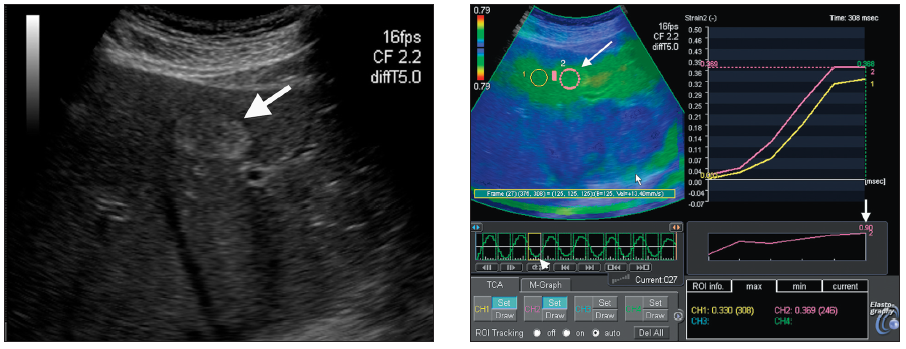
\includegraphics[width=1\textwidth]{rysunki/obrazyWE}
%	\caption{Obraz ultrasonograficzny (po lewej) oraz odpowiadaj�cy mu obraz elastografii typu strain~\cite{Onur}}
%	\label{obrazyWE}
%\end{figure}

\begin{figure} [H]
	\centering
	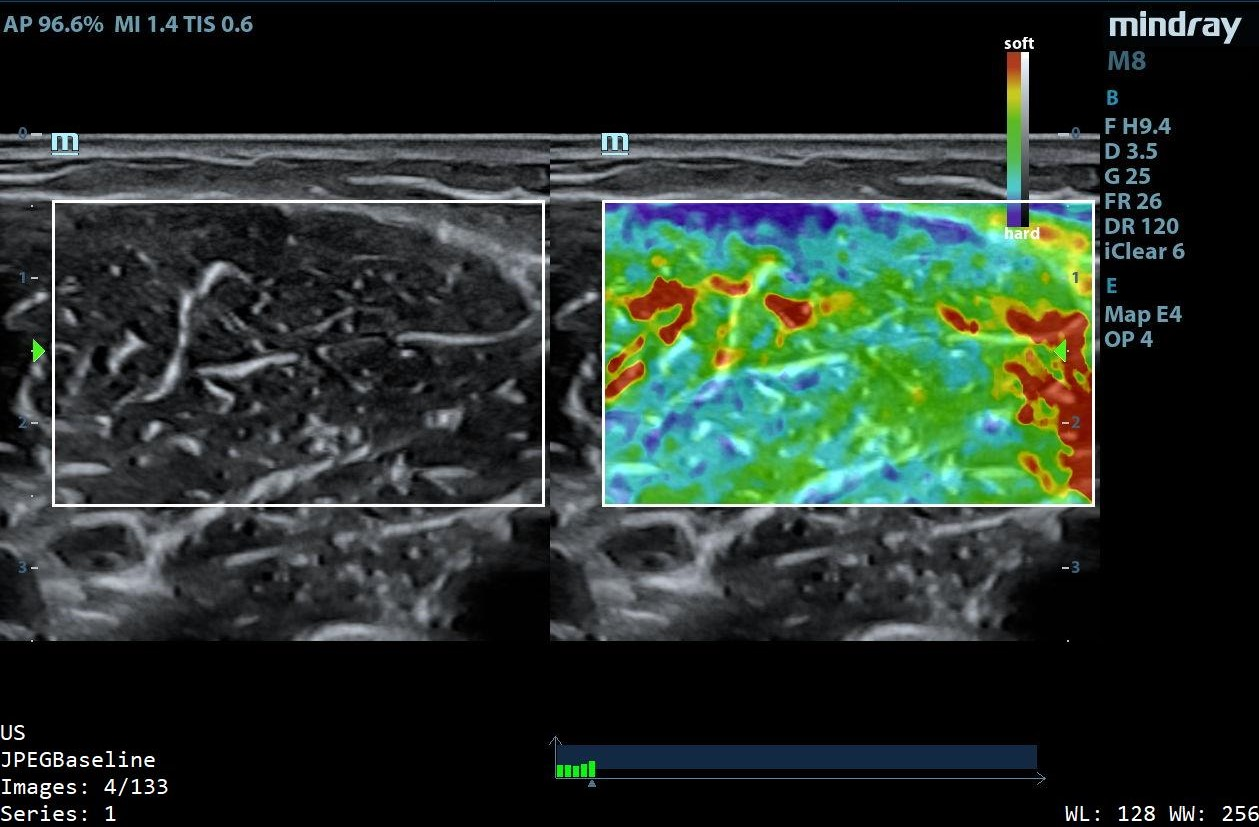
\includegraphics[width=0.7\textwidth]{rysunki/elasto}
	\caption{Obraz ultrasonograficzny (po lewej) oraz odpowiadaj�cy mu obraz elastografii}
	\label{obrazyWE}
\end{figure}

Odkszta�ceniem liniowym $\epsilon$ nazywa si� stosunek zmiany d�ugo�ci tkanki podczas deformacji, w odniesieniu do d�ugo�ci pierwotnej. Zale�no�� t� opisuje wz�r \cite{Cygan}:

\begin{equation}
\epsilon = \dfrac{L-{L}_0}{{L}_0}.
\end{equation}

Natomiast napr�enie jest stosunkiem si�y do pola przekroju badanej tkanki (obiektu) i opisuje j� zale�no�� \cite{Cygan}:

\begin{equation}
\sigma = \dfrac{F}{S}
\end{equation}

\section{Rozwi�zania alternatywne}
TO DO

\section{Cel pracy}
Celem pracy jest opracowanie oraz implementacja metodologii mapowania zmian odkszta�ce� w tkankach mi�kkich w badaniach ultrasonograficznych. Zak�ada si�, �e opracowana metoda b�dzie wykorzystywa�a �ledzenie cech obrazu w sekwencji obraz�w USG podczas ucisku tkanki. Przyk�adem badania, z jakim b�dzie mo�na por�wna� wyniki otrzymane przez stworzony algorytm jest elastografia typu Strain.
%\section{Uk�ad pracy}
%%%%%%%%%%%%%%%%%%%%%%%%%%%%%%%%%%%%%%%%%%%%%%%%%%%%%%%%%%%%%%%%%%%%%%%%%%%%%%%%%%%%%%%%%%%%%%%%%%%%%%%%%%%%%%%%%%%%%%%%%%%%%%%%%%%%%%%%%%%%%%%%%%%%%%%%%%%%%%%%%%%%%%%
\chapter{Metodologia}\label{Chapter_Metodologia}

\section{Opis stanowiska badawczego}\label{stanowisko}
Stanowisko mia�o na celu umo�liwienie rejestracji obraz�w ultrasonograficznych, przedstawiaj�cych ... . Do wykonania symulacji badania konieczne by�o ... . uproszczony schemat wykorzystanego stanowiska zosta� przedstawiony na Rysunku .... W jego sk�ad wchodzi�y jednostki takie jak:
\begin{itemize}
	\item ...
	\item ...
\end{itemize}

\section{Akwizycja danych}
Rejestracja danych zosta�a przeprowadzona na przedstawionym w sekcji \ref{stanowisko} stanowisku badawczym. Do akwizycji obraz�w wykorzystano urz�dzenie Mindray UMT-500Plus wraz z g�owicami: liniow� L13-3s oraz konweksow� C5-1s. Serie obrazowe zosta�y zapisane z wykorzystaniem standardu DICOM. 

\subsubsection{Przyk�adowe obrazy}
TO DO

%\begin{figure}[H]
% \subfloat[Podpis 1\label{f1:c1}]{
\includegraphics[width=0.45\textwidth]{logoPS}} \; % <--- to daje odst�p w poziomie; \\ daje now� linijk�
% \subfloat[Podpis 2\label{f1:c2}]{
\includegraphics[width=0.45\textwidth]{logoRIB}} 
%  \caption{Podpis ca�o�ci nawi�zuj�cy do podpisu \protect\subref{f1:c1}.\label{f1}} % wykorzystanie subref mo�e wymaga� dodania \protect !!!
%\end{figure}

%%%%%%%%%%%%%%%%%%%%%%%%%%%%%%%%%%%%%%%%%%%%%%%%%%%%%%%%%%%%%%%%%%%%%%%%%%%%%%%%%%%%%%%%%%%%%%%%%%%%%%%%%%%%%%%%%%%%%%%%%%%%%%%%%%%%%%%%%%%%%%%%%%%%%%%%%%%%%%%%%%%%%%%
%\chapter{Specyfikacja wewn�trzna}

%\section{Specyfikacja interfejsu programistycznego}
%\lstset{ %
%numbers=left, 
%}

%\begin{lstlisting}
%kod
%\end{lstlisting}

%\begin{itemize}
% \item Parametry:
%    \begin{description}
%    \item[ile] okre�la ile rezy nale�y losowa� przed zwr�ceniem liczby,
%    \item[min] definiuje warto�� minimaln�,
%    \item[max] definiuje warto�� minimaln�,
%    \end{description}
% \item Warto�� zwracana: wylosowana liczba
% \item B��dy: w~przypadku, gdy \lstinline{ile} $< 0$, zg�aszany jest wyj�tek \lstinline{WrongIleException}
%\end{itemize}

%\begin{lstlisting}[numbers=right, numbersep=-5pt]%, stepnumber=2]
%...
%double x = 2 ^ 1023-3 / 22;
%int z = (int)x; 
%p = x - z;
%...
%\end{lstlisting}
%%%%%%%%%%%%%%%%%%%%%%%%%%%%%%%%%%%%%%%%%%%%%%%%%%%%%%%%%%%%%%%%%%%%%%%%%%%%%%%%%%%%%%%%%%%%%%%%%%%%%%%%%%%%%%%%%%%%%%%%%%%%%%%%%%%%%%%%%%%%%%%%%%%%%%%%%%%%%%%%%%%%%%%
%\chapter{Specyfikacja zewn�trzna}

%%%%%%%%%%%%%%%%%%%%%%%%%%%%%%%%%%%%%%%%%%%%%%%%%%%%%%%%%%%%%%%%%%%%%%%%%%%%%%%%%%%%%%%%%%%%%%%%%%%%%%%%%%%%%%%%%%%%%%%%%%%%%%%%%%%%%%%%%%%%%%%%%%%%%%%%%%%%%%%%%%%%%%%
%\chapter{Rezultaty}

%%%%%%%%%%%%%%%%%%%%%%%%%%%%%%%%%%%%%%%%%%%%%%%%%%%%%%%%%%%%%%%%%%%%%%%%%%%%%%%%%%%%%%%%%%%%%%%%%%%%%%%%%%%%%%%%%%%%%%%%%%%%%%%%%%%%%%%%%%%%%%%%%%%%%%%%%%%%%%%%%%%%%%%
%\chapter{Podsumowanie}












\begin{thebibliography}{0.9}
\bibitem{Barr} Richard G. Barr, Zheng Zhang, \textit{Shear-wave elastography of the breast: value of a quality measure and comparison with strain elastography}, Radiology, Tom 275, Numer 1, 2015, s. 45-53.

\bibitem{Carlsen} Jonathan F. Carlsen, Caroline Ewertsen, Lars L�nn, Michael B. Nielsen, \textit{Strain elastography ultrasound: an overview with emphasis on breast cancer diagnosis, Diagnostics}, Tom 3, 2013, s. 117-125.

\bibitem{Chang}	Jung Min Chang, Jae-Kyung Won, Kyoung-Bun Lee, In Ae Park, Ann Yi, Woo Kyung Moon, \textit{Comparison of Shear-wave and strain ultrasound elastography in the differentiation of begin and malignant breast lesions}, American Roentgen Ray Society, Tom 201, 2013, s. 347-356.

\bibitem{Ferraioli}	Giovanna Ferraioli, Carmine Tinelli, Antonello Malfitano, Barbara Dal Bello, Gaetano Filice, Carlo Filice, \textit{Performance of real-time strain elastography, transient elastography, and aspartate-to-platelet ratio index in the assessment of fibrosis in chronic hepatitis C}, American Roentgen Ray Society, Tom 199, 2012, s. 19-25.

\bibitem{Dietrich} Christoph F. Dietrich, Richard G. Barr, Andr� Farrokh, Manjiri Dighe, Michael Hocke, Christian Jenssen, Yi Dong, Adrian Saftoiu, Roald Flesland Havre, \textit{Strain elastography � how to do it?}, Ultrasound int Open, Tom 3, 2017, s. 137-149. 

\bibitem{Onur}	Mehmet Ruhi Onur, Ahmet Kursad Poyraz, Esra Ercin Ucak, Zulkif Bozgeyik, Ibrahim Hanifi �zercan, Erkin Ogur, \textit{Semiquntitative strain elastography of liver masses}, American Institute of Ultrasound in Medicine | J Ultrasound Med, Tom 31, 2012, s. 1061-1067.

\bibitem{Cygan}	Szymon Cygan, \textit{Metoda wyznaczania przemieszcze� i odkszta�ce� dla potrzeb elastografii w warunkach znacznych odkszta�ce� tkanek}, Rozprawa doktorska, Politechnika Warszawska, Wydzia� Mechatroniki, 2011.

\bibitem{Thitaikumar} Arun Thitaikumar, Louise M Mobbs, Christina M Kraemer-Chant, Brian S Garra, Jonathan Ophir, \textit{Breast tumor classification using axial shear strain elastography: a feasibility study}, Physics in Medicine and Biology, Tom 53, 2008, s. 4809-4823.

\bibitem{Grajo}	Joseph R. Grajo, Richard G. Barr, \textit{Strain elastography for prediction of breast cancer tumor grades}, American Institute of Ultrasound in Medicine | J Ultrasound Med, Tom 33, 2014, s. 278-297.

\bibitem{Fedak} Andrzej Fedak, \textit{Badania ultrasonograficzne: elastografia ultrasonograficzna}, In�ynier i Fizyk Medyczny, Tom 8, 2019, s. 167-170.

\bibitem{Drakonaki} Elena Drakonaki, \textit{Elastografia w obrazowaniu �ci�gien i mi�ni}, Journal of Ultrasonography, Tom 12, 2012, s. 214-225.

\bibitem{Batko} Tomasz Batko, \textit{Ocena przydatno�ci ,,jako�ciowej elastografii ultrasonograficznej czasu rzeczywistego" w r�nicowaniu pomi�dzy prawid�owymi i patologicznymi w�z�ami ch�onnymi szyjnymi u dzieci i m�odzie�y}, Rozprawa doktorska, Gda�ski Uniwersytet Medyczny, 2014.

\bibitem{Maurice} Maurice, R. L., Ohayon, J., Fretigny, Y., Bertrand, M., Soulez, G., Cloutier, G., Noninvasive \textit{Vascular Elastography: Theoretical Framework}, IEEE Transactions on Medical Imaging, Tom 23, Numer 2, 2004, s. 164�180.

\bibitem{Korukonda} Korukonda, S., Doyley, M., \textit{Visualizing the radial and circumferential strain distribution within vessel phantoms using synthetic-aperture ultrasound elastography}, IEEE Transactions on Ultrasonics, Ferroelectrics and Frequency Control, Tom 59, Numer 8, 2012, s. 1639�1653.

\bibitem{Nayak} Nayak, R., Huntzicker, S., Ohayon, J., Carson, N., Dogra, V., Schifitto, G., Doyley, M. M., \textit{Principal Strain Vascular Elastography: Simulation and Preliminary Clinical Evaluation}, Ultrasound in Medicine \& Biology, Tom 43, Numer 3, 2017, s. 682�699.

\bibitem{Maurice2} Maurice, R. L., Daronat, M., Ohayon, J., Stoyanova, �., Foster, F. S., Cloutier, G., \textit{Non-invasive high-frequency vascular ultrasound elastography}, Physics in Medicine and Biology, Tom 50, Numer 7, 2005, s. 1611�1628.

\bibitem{WHO} \textit{Manual of diagnostic ultrasound. Vol. 1. -- 2nd ed}, red. Harald Lutz, Elisabetta Buscarini, World Health Organization, 2011.

\end{thebibliography}

%\appendix  % <--- zaczynaj� si� dodatki; jak nazywa si� rozdzia� -> szuka� appendixname powy�ej
%\chapter{Dodatek A}
W dodatku umieszczamy opis ewentualnych znanych algorytm�w, z kt�rych korzystamy proponuj�c w�asn� metodologi�, opisan� w rozdziale~\ref{Chapter_Metodologia}. Wykaz pozycji literaturowych tworzymy w oddzielnym pliku \texttt{Praca.bib}. Chc�c si� odwo�a� w tek�cie do wybranej pozycji bibliograficznej korzystamy z komendy \texttt{cite}. Efekt jej u�ycia dla kilku pozycji jednocze�nie to~\cite{Tadeusiewicz,Malina,Nieniewski_Morfologia}.

%%%%%%%%%%%%%%%%%%%%%%%%%%%%%%%%%%%%%%%%%%%%%%%%%%%%%%%%%%%%%%%%%%%%%%%%%%%%%%%%%%%%%%%%%%%%%%%%%%%%%%%%%%%%%%%%%%%%%%%%%%%%%%%%%%%%%%%%%%%%%%%%%%%%%%%%%%%%%%%%%%%%%%%
\chapter{Dodatek B}
Podstawowe kwestie techniczne dotycz�ce wzor�w, rysunk�w, tabel poni�ej.

Wzory tworzymy w �rodowisku \texttt{equation}. Chc�c odwo�a� si� do wybranego wzoru gdzie� w tek�cie nale�y nada� mu stosown�, niepowtarzaln� i jednoznaczn� etykiet�, po ty by m�c np. napisa� zdanie: ze wzoru~\ref{Wzor_Dodawanie} wynika \ldots
\begin{equation}\label{Wzor_Dodawanie}
	c = a + b
\end{equation}

Wzory z�o�one, charakteryzuj�ce si� przypisaniem warto�ci zmiennej w pewnych okoliczno�ciach tworzymy przy u�yciu otoczenia \texttt{eqnarray}. Odwo�anie do wzoru jak wcze�niej. 
\begin{eqnarray}\label{equ_progowanie}
    BW & = & \left \{
    \begin{array}{ll}
      1, & I(x,y) \geq T \\
      0, & I(x,y) < T\\
    \end{array}
    \right.,
\end{eqnarray}

% \subsection{Usuwanie numeracji przy r�wnaniach}

Numeracj� r�wna� mo�na tymczasowo (w~danej linijce) wy��czy� poprzez u�ycie $\backslash{}nonumber$
\begin{eqnarray}
	a_i = a_{i-1}+a_{i-2}\nonumber \\ % w tej linijce nie ma numeru
              +a_{i-3}
\end{eqnarray}


\section{Wstawianie rysunk�w}
Rysunki umieszczamy w otoczeniu \texttt{figure}, centruj�c je w poziomie komend� \texttt{centering}. Rozmiary rysunku ustalamy w komendzie \texttt{includegraphics} dobieraj�c wielko�� wzgl�dem rozmiaru strony lub bezwzgl�dnie np. w cm. Ponadto najpierw zapowiadamy pojawienie si� rysunku w tek�cie (czyli np. Na rysunku (Rys~\ref{Rysunek_LogoIB}) pracy, a dopiero p�niej wstawiamy sam rysunek. Dodatkowo sterowa� mo�emy umiejscowieniem rysunku na stronie dzi�ki parametrom \texttt{[!htb]} okre�laj�cym miejsce. Odpowiednio s� to: \texttt{here}, \texttt{top}, \texttt{bottom}. 
\begin{figure}[!htb]
	\centering
	
\includegraphics[width=.35\textwidth]{logoRIB}
	\caption{Logo Wydzia�u In�ynierii Biomedycznej.}\label{Rysunek_LogoIB}
\end{figure}

Do��czaj�c rysunki nie trzeba podawa� rozszerzenia (wr�cz jest to odradzane). Je�li rysunki znajduj� si� w~katalogu \emph{rysunki}, nie trzeba r�wnie� podawa� �cie�ki do nich.

\section{Wstawianie tabelek}
Analogicznie post�pujemy z tabelkami, z t� r�nic� �e tworzymy j� w otoczeniu \texttt{table}. W nim natomiast sam� tabel� definiujemy albo w �rodowisku \texttt{tabular}, albo \texttt{tabularx}. Podobnie z odwo�aniami w tek�cie: najpierw odwo�anie w Tab.~\ref{Tabelka_Tabela}, a dopiero p�niej sama tabela.
\begin{table}[!htb]
	\centering
	\topcaption{Opis nad tabelk�.}\label{Tabelka_Tabela}
	\begin{tabular}{|c|c|c|c|} \hline \hline 
		Kolumna 1 & Kolumna 2 & Kolumna 3 & Kolumna 4 \\ \hline
		Wiersz 1 & & & \\ \hline
		Wiersz 2 & & & \\ \hline
		Wiersz 3 & & & \\ \hline
		& & & \\ \hline
		& & & \\ \hline
	\end{tabular}
\end{table}

%%%%%%%%%%%%%%%%%%%%%%%%%%%%%%%%%%%%%%%%%%%%%%%%%%%%%%%%%%%%%%%%%%%%%%%%%%%%%%%%%%%%%%%%%%%%%%%%%%%%%%%%%%%%%%%%%%%%%%%%%%%%%%%%%%%%%%%%%%%%%%%%%%%%%%%%%%%%%%%%%%%%%%%
\chapter{Kwestie edytorskie}
Zbi�r zasad pomocnych przy redagowaniu tekstu pracy wystarczaj�co szczeg�owo przedstawia ksi��ka~\cite{Chwalowski}.

Uwaga! Pisz�c prac� nale�y zwr�ci� uwag� na nast�puj�ce kwestie:
\begin{enumerate}
	\item Prace piszemy w formie bezosobowej.
	\item Unikamy okre�le� potocznych, spolszcze� funkcjonuj�cych codziennej mowie itp.
	\item Pos�uguj�c si� znanymi nam (a nie czytelnikowi) has�ami (r�wnie� skr�tami, akronimami) najpierw je definiujemy i~t�umaczymy, a~dopiero p�niej traktujemy za znane.
	\item Podpisy pod rysunkami lub nad tabelami traktujemy jak zdania, a wi�c powinny stanowi� sp�jn� ca�o�� oraz powinny zosta� zako�czone kropk�.
	\item Podobnie wypunktowania (po dwukropku kolejne punkty pisane ma�ymi literami, oddzielane przecinkami, ostatni zako�czony kropk� o ile ko�czy zdanie).
	\item Do ka�dego rysunku, tabeli, pozycji bibliograficznej musi istnie� odwo�anie w tek�cie pracy, przy czym do pierwszych dw�ch musi si� ono pojawi� zanim umie�cimy rysunek/tabel�.
\end{enumerate}


\clearpage \addcontentsline{toc}{chapter}{\bibname}
%\bibliography{Praca}


\end{document}
